\documentclass[11pt,a4paper]{article}

% ------------------------------------------------------------------
% Packages (same style as the setup guide and the project log)
% ------------------------------------------------------------------
\usepackage[T1]{fontenc}
\usepackage[utf8]{inputenc}
\usepackage{lmodern}
\usepackage[margin=2.5cm]{geometry}
\usepackage{booktabs}
\usepackage{tabularx}
\usepackage{array}
\usepackage{longtable}
\usepackage{xcolor}
\usepackage{enumitem}
\usepackage{fancyhdr}
\usepackage{titlesec}
\usepackage{listings}
\usepackage{float}
\usepackage{amssymb}
\usepackage{tikz}
\usetikzlibrary{positioning,arrows.meta}
\usepackage{xurl}
\usepackage{hyperref}

\hypersetup{colorlinks=true, linkcolor=blue!50!black, urlcolor=blue!50!black}

\definecolor{codebg}{gray}{0.96}
\definecolor{notebg}{RGB}{255,246,228}
\definecolor{noteframe}{RGB}{200,110,0}
\definecolor{tipbg}{RGB}{232,242,252}
\definecolor{tipframe}{RGB}{42,120,214}
\definecolor{okgreen}{RGB}{0,120,60}

\lstset{
  basicstyle=\ttfamily\small,
  backgroundcolor=\color{codebg},
  frame=single,
  rulecolor=\color{gray!40},
  breaklines=true,
  columns=fullflexible,
  keepspaces=true,
  showstringspaces=false
}

\newcommand{\code}[1]{\texttt{#1}}
\newcommand{\bs}{\textbackslash\allowbreak{}}
\let\oldunderscore\_
\renewcommand{\_}{\oldunderscore\allowbreak{}}
\newcommand{\pld}[1]{\code{C:\bs PLD\bs #1}}
\newcommand{\out}[1]{\code{C:\bs PLD\_out\bs #1}}
\newcommand{\menu}[1]{\textsf{#1}}
\newcommand{\checkbox}{$\square$\ }
\newcolumntype{Y}{>{\raggedright\arraybackslash}X}

\newcommand{\important}[1]{%
  \par\smallskip\noindent
  \fcolorbox{noteframe}{notebg}{\parbox{\dimexpr\linewidth-2\fboxsep-2\fboxrule\relax}{\small\textbf{Important.} #1}}%
  \par\smallskip}
\newcommand{\tip}[1]{%
  \par\smallskip\noindent
  \fcolorbox{tipframe}{tipbg}{\parbox{\dimexpr\linewidth-2\fboxsep-2\fboxrule\relax}{\small\textbf{Why.} #1}}%
  \par\smallskip}

\setlength{\emergencystretch}{3em}
\setlength{\parskip}{4pt}
\setlength{\parindent}{0pt}

\pagestyle{fancy}
\fancyhf{}
\lhead{\small TeraNova -- FPGA Acceleration}
\rhead{\small Board guide -- K.~Janssen (4994817)}
\cfoot{\small\thepage}
\renewcommand{\headrulewidth}{0.4pt}

\titleformat{\subsection}{\normalfont\large\bfseries}{\thesubsection}{1em}{}

% ------------------------------------------------------------------
\begin{document}

\begin{titlepage}
\centering
\vspace*{3cm}
{\LARGE\bfseries Board Guide\par}
\vspace{0.5cm}
{\Large Building and Measuring Every Rung of the\\Improvement Ladder on the ZCU102\par}
\vspace{0.3cm}
{\large TeraNova -- FPGA Acceleration\par}
\vspace{2cm}
\begin{tabular}{@{}ll@{}}
\textbf{Author}          & Kai Janssen (4994817) \\
\textbf{Version}         & 30 October 2026 \\
\textbf{Board}           & AMD ZCU102 (Zynq UltraScale+ \code{xczu9eg-ffvb1156-2-e}) \\
\textbf{Tools}           & Vivado / Vitis 2025.1.1, git, PuTTY \\
\textbf{Repository}      & \code{github.com/GiganticGnu/TeraNova-FPGA}, at \code{C:\bs PLD} \\
\end{tabular}
\vfill
{\small Board details in this guide come from the ZCU102 Evaluation Board User Guide (UG1182) and the Zynq UltraScale+ MPSoC Embedded Design Tutorial (UG1209); see the references at the end.\par}
\end{titlepage}

\tableofcontents
\newpage

% ==================================================================
\section{What this guide is for}
% ==================================================================
The accelerator is being improved step by step. Every step is one \emph{rung} of the improvement ladder, and every rung is stored as its own git branch. Each rung contains all earlier rungs plus one new change. To see what each change brings, the rungs are measured on the board \textbf{one at a time, in this order}:

\begin{table}[H]
\centering
\small
\begin{tabularx}{\textwidth}{@{}clYlr@{}}
\toprule
\textbf{Rung} & \textbf{Git ref} & \textbf{What changes} & \textbf{Application} & \textbf{PL time (sim.)} \\
\midrule
0 & tag \code{baseline-1} (\code{main}) & Nothing: the restored design, the reference & baseline & 1012\,\textmu s \\
1 & \code{partitioner-v5b} & Partitioner fetches one element per cycle & baseline & 272\,\textmu s \\
2 & \code{writer-fix} & Result writer no longer waits for every write response & baseline & 271\,\textmu s \\
3 & \code{partitioner-v6} & Partitioner copies A and B on chip once, reuses them 10$\times$ & baseline & 101\,\textmu s \\
4 & \code{burst-datapath} & PL reads A/B from and writes C to the processor's DDR; no BRAMs & burst & 101\,\textmu s \\
\bottomrule
\end{tabularx}
\caption{The five rungs. ``PL time'' is the simulated start-to-\code{done} time at 100\,MHz for the nominal memory latency (Section~\ref{sec:expected} gives the full expected range). The application is already the right one on every branch.}
\label{tab:rungs}
\end{table}

For every rung the same three phases are done (Figure~\ref{fig:phases}). Phase~A needs the Vivado licence, so it runs on Badr's laptop. Phases B and C need no licence and can be done on any PC that has the tools and is connected to the board.

\begin{figure}[H]
\centering
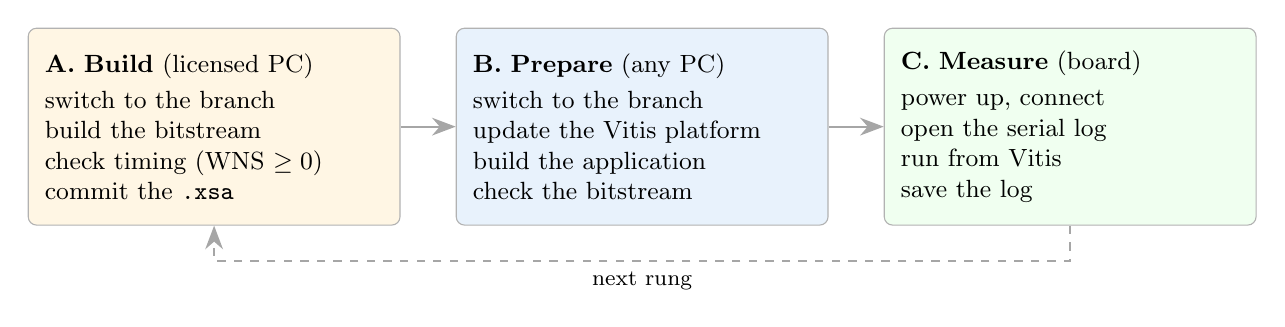
\begin{tikzpicture}[
  box/.style={draw=gray!60, rounded corners=3pt, fill=#1, align=left, text width=4.3cm, minimum height=2.5cm, inner sep=6pt, font=\small},
  arr/.style={-{Stealth[length=3mm]}, thick, gray!70}]
\node[box=notebg] (a) {\textbf{A. Build} (licensed PC)\\[2pt]switch to the branch\\build the bitstream\\check timing (WNS $\geq 0$)\\commit the \code{.xsa}};
\node[box=tipbg, right=0.7cm of a] (b) {\textbf{B. Prepare} (any PC)\\[2pt]switch to the branch\\update the Vitis platform\\build the application\\check the bitstream};
\node[box=green!6, right=0.7cm of b] (c) {\textbf{C. Measure} (board)\\[2pt]power up, connect\\open the serial log\\run from Vitis\\save the log};
\draw[arr] (a) -- (b);
\draw[arr] (b) -- (c);
\draw[arr, dashed] (c.south) -- ++(0,-0.45) -| node[pos=0.25, below, font=\footnotesize, text=black] {next rung} (a.south);
\end{tikzpicture}
\caption{The three phases, repeated for every rung.}
\label{fig:phases}
\end{figure}

\important{Never mix rungs. The hardware file (\code{.xsa}), the Vitis platform and the application must all come from the \emph{same} branch. A run with a bitstream of one rung and the platform of another either fails or, worse, gives believable but wrong numbers. Every phase below starts with a check of the branch for exactly that reason.}

% ==================================================================
\section{One-time preparation}\label{sec:once}
% ==================================================================
\subsection{Software on the PC that drives the board}
\begin{enumerate}
  \item \textbf{Vivado and Vitis 2025.1.1}, installed in \code{C:\bs Xilinx\bs 2025.1.1} with Zynq UltraScale+ MPSoC support. Only this version: 2025.1 locks every IP of the project.
  \item \textbf{JTAG cable drivers.} Run once, as administrator:
\begin{lstlisting}
C:\Xilinx\2025.1.1\data\xicom\cable_drivers\nt64\install_drivers_wrapper.bat
\end{lstlisting}
  \item \textbf{USB-UART driver.} The board's serial port is a Silicon Labs CP2108 quad USB-UART bridge. Install the \emph{CP210x Universal Windows Driver} (VCP driver) from the Silicon Labs website if Windows does not install it by itself.
  \item \textbf{git} (Git for Windows, includes Git Bash) and \textbf{PuTTY} (serial terminal that can write a log file).
\end{enumerate}

\subsection{The repository}
The project must be at exactly \code{C:\bs PLD}: the Vivado project and the Vitis workspace contain absolute paths. If \code{C:\bs PLD} does not exist yet, open Git Bash and run:
\begin{lstlisting}
git clone https://github.com/GiganticGnu/TeraNova-FPGA.git /c/PLD
\end{lstlisting}
If it already exists, bring it up to date:
\begin{lstlisting}
cd /c/PLD
git status          # must say "nothing to commit, working tree clean"
git fetch --all --tags
\end{lstlisting}
Finally, make a folder for the results, outside the repository: \out{}. Every rung gets its own sub-folder, named after the rung: \code{0\_baseline}, \code{1\_partitioner\_v5b}, \code{2\_writer\_fix}, \code{3\_partitioner\_v6}, \code{4\_burst\_datapath}.

% ==================================================================
\section{The board}\label{sec:board}
% ==================================================================
\subsection{The parts you use}
Figure~2-1 of UG1182 shows where everything is; the reference designators are also printed on the board itself.

\begin{longtable}{@{}p{0.17\textwidth}p{0.27\textwidth}p{0.48\textwidth}@{}}
\toprule
\textbf{Part} & \textbf{What it is} & \textbf{What you do with it} \\
\midrule
\endhead
\code{J52} & 12\,V power connector & Plug in the board's own 12\,V supply (6-pin connector). Use no other supply. \\
\code{SW1} & Power on/off slide switch & Switch the board on and off. Always switch off before you change cables or switches. \\
\code{SW6} & 4-pole DIP switch: boot mode & Must be set to \textbf{JTAG}: all four switches \textbf{ON} (mode pins 0000). This is also the factory default. In JTAG mode the processor waits for Vitis to load the program; it does not boot from the SD card or flash. \\
\code{J2} & Micro-USB: JTAG (on-board Digilent USB-to-JTAG module) & Cable 1 to the PC. Vitis uses it to program the FPGA and load the program. \\
\code{J83} & Micro-USB: USB-UART (CP2108, 4 channels) & Cable 2 to the PC. Channels 0 and 1 are the processor's UARTs, channel 2 goes to the PL, channel 3 to the board's system controller. Our program prints on \textbf{channel 0} (PS UART0). \\
\code{DS32} & Green LED ``DONE'' & Lights when the FPGA has been programmed (``bit file download is complete''). \\
Green power LEDs & e.g.\ \code{DS21}--\code{DS26}, \code{DS19}, \code{DS31} & Light when the supply rails are on. \\
\code{DS35}, \code{DS36} & Red LEDs: PS error, power-on reset & Must be \textbf{off} while the board runs. \\
\code{SW4}, \code{SW3} & Push buttons: power-on reset (\code{POR\_B}), system reset (\code{SRST}) & Not needed for this guide; use \code{SW1} to restart the board instead. \\
\bottomrule
\end{longtable}

\important{The board is sensitive to static electricity. Touch a grounded metal object before you handle it, hold it by the edges, and keep it on its standoffs on a non-conductive surface. Never connect or disconnect anything while \code{SW1} is on.}

\subsection{Connecting and switching on}\label{sec:connect}
Do this once at the start of a board session.
\begin{enumerate}
  \item With \code{SW1} \textbf{off}: check that \code{SW6} is set to JTAG (all four ON).
  \item Connect the 12\,V supply to \code{J52}.
  \item Connect micro-USB cable~1 from \code{J2} (JTAG) to the PC, and cable~2 from \code{J83} (UART) to the PC.
  \item Switch \code{SW1} on. The fan starts, the green power LEDs light, and the red LEDs \code{DS35}/\code{DS36} stay off. \code{DS32} (DONE) is still off: no bitstream has been loaded yet.
  \item \textbf{Find the serial port.} Open the Windows \menu{Device Manager} $\rightarrow$ \menu{Ports (COM \& LPT)}. You see four entries ``Silicon Labs Quad CP2108 USB to UART Bridge: Interface 0'' to ``Interface 3'', each with a COM number. \textbf{Interface~0 is PS UART0}, where the program prints. Write down its COM number (UG1209: ``MPSoC UART-0 corresponds to the COM port with Interface-0''). If you see no CP2108 entries, the driver is missing (Section~\ref{sec:once}).
  \item \textbf{Check the JTAG connection} (only needed the first time, or when something fails). In Vivado: \menu{Open Hardware Manager} $\rightarrow$ \menu{Open target} $\rightarrow$ \menu{Auto Connect}. The hardware tree must show the \code{xczu9\_0} device. Then \textbf{close the Hardware Manager}: as long as it is open it holds the JTAG cable and Vitis cannot use it.
\end{enumerate}

\subsection{The serial log (PuTTY)}\label{sec:putty}
Everything the program prints is the measurement, so it is written to a file directly.
\begin{enumerate}
  \item Start PuTTY. \menu{Session}: Connection type \menu{Serial}, Serial line \code{COMx} (the Interface~0 port), Speed \code{115200}.
  \item \menu{Connection $\rightarrow$ Serial}: 8 data bits, 1 stop bit, parity \menu{None}, flow control \menu{None}.
  \item \menu{Session $\rightarrow$ Logging}: select \menu{Printable output}; Log file name \out{<rung>\bs board\_log.txt}, for example \out{0\_baseline\bs board\_log.txt}; select \menu{Ask the user} for an existing file.
  \item Click \menu{Open}. The window stays empty until the program runs.
\end{enumerate}
Save these settings under a name (\menu{Session $\rightarrow$ Saved Sessions}, e.g.\ \code{ZCU102}); then only the log file name has to be changed per rung. The Vitis \menu{Serial Monitor} works too, but it does not write a log file.

% ==================================================================
\section{Phase A -- Build a rung (licensed PC)}\label{sec:build}
% ==================================================================
This phase turns the design of one branch into a hardware file, \code{interrupt\_rerun.xsa}, which contains the bitstream. It is the only phase that needs the licence. Do the rungs in ladder order.

\begin{enumerate}
  \item \textbf{Start clean.} Close Vivado and Vitis. In Git Bash:
\begin{lstlisting}
cd /c/PLD
git status                # must be clean; if not, see the note below
git fetch --all --tags
\end{lstlisting}
  \item \textbf{Switch to the rung.}
\begin{lstlisting}
git switch main               # rung 0  (main = tag baseline-1)
git switch partitioner-v5b    # rung 1
git switch writer-fix         # rung 2
git switch partitioner-v6     # rung 3
git switch burst-datapath     # rung 4
git pull                      # then: get the latest commit of that branch
git log -1 --oneline          # check the commit (table below)
\end{lstlisting}
  Only the line of the rung you build, of course.
  \textbf{Expected commit} (\code{git log -1} shows this one, or a later ``Build of rung'' commit on top of it):\par
  {\small
  \begin{tabularx}{\linewidth}{@{}cllY@{}}
  \toprule
  \textbf{Rung} & \textbf{Branch} & \textbf{Commit} & \textbf{Message starts with} \\
  \midrule
  0 & \code{main} & \code{3c52095} & Measurement app, simulation testbenches \\
  1 & \code{partitioner-v5b} & \code{5c49045} & Partitioner v5b (pipelined fetch) \\
  2 & \code{writer-fix} & \code{70ba245} & Writer fix: explicit bursts \\
  3 & \code{partitioner-v6} & \code{b056560} & Partitioner v6: on-chip copy \\
  4 & \code{burst-datapath} & \code{b99091c} & Rung 4: burst data path \\
  \bottomrule
  \end{tabularx}\par}
  \item \textbf{Open the project.} Start Vivado \textbf{2025.1.1} and open \pld{S7\_integration\bs S7\_integration.xpr}. The many \code{[Board 49-26]} warnings and the ``generated file not found \ldots\ regenerate'' warnings are normal. \menu{Reports $\rightarrow$ Report IP Status}: nothing may be locked. (On rung~4 the partitioner is \code{partitioner\_v7\_0}, an RTL module; that is correct.)
  \item \textbf{Build.} In the Tcl Console:
\begin{lstlisting}
source C:/PLD/scripts/3_build_and_export.tcl
\end{lstlisting}
  This takes a long time (synthesis, implementation, bitstream). At the end it prints \code{Worst negative slack: \ldots\ ns} and writes \pld{S7\_integration\bs interrupt\_rerun.xsa}.
  \item \textbf{Check timing.} The worst negative slack (WNS) must be \textbf{$\geq 0$}. If it is negative, timing is not met: stop here and report it. Do not run this rung on the board.
  \item \textbf{Save the reports.} In the Tcl Console (use the folder of this rung):
\begin{lstlisting}
file mkdir C:/PLD_out/0_baseline
open_run impl_1
report_utilization    -file C:/PLD_out/0_baseline/utilization.txt
report_timing_summary -file C:/PLD_out/0_baseline/timing.txt
file copy -force C:/PLD/S7_integration/interrupt_rerun.xsa C:/PLD_out/0_baseline/
\end{lstlisting}
  \item \textbf{Close Vivado}, then commit only the hardware file, and throw away everything else the build changed:
\begin{lstlisting}
git add S7_integration/interrupt_rerun.xsa
git commit -m "Build of rung 0 (WNS 0.123 ns)"
git push
git restore .
git status                # must be clean again
\end{lstlisting}
  Put the real rung number and WNS in the message.
\end{enumerate}
\tip{The \code{.xsa} is tracked by git. Committing it to the rung's own branch makes the build available to everyone: phases B and C can then be done on any PC, without the licence and without copying files by hand. The other files the build touches (the project file, IP state) are not needed and are restored, so that the next \code{git switch} works.}

\important{If \code{git status} is not clean before you start, or \code{git switch} says ``Your local changes \ldots\ would be overwritten'', do \emph{not} force anything. Changes left over from a build are thrown away with \code{git restore .}; anything else, ask first.}

% ==================================================================
\section{Phase B -- Prepare Vitis for a rung (no licence)}\label{sec:prepare}
% ==================================================================
\begin{enumerate}
  \item \textbf{Switch to the rung and get its build.} Close Vitis. In Git Bash:
\begin{lstlisting}
cd /c/PLD
git status                # clean
git switch writer-fix     # the branch of this rung (see Phase A)
git pull
git log -1 --oneline -- S7_integration/interrupt_rerun.xsa
\end{lstlisting}
  The last command must show \textbf{``Build of rung $N$''} for \emph{this} rung. If it shows \code{2e936e3 Baseline: restored working build}, this branch has not been built yet: the \code{.xsa} is still the previous group's file. Do not continue with that file.
  \item \textbf{Check the application.} Open \pld{S7\_integration\_vit\bs interrupt\_rerun\_test\bs src\bs helloworld.c}. Line~3 must say \code{BASELINE MEASUREMENT VERSION} for rungs 0--3, or \code{LADDER STEP 4: BURST DATA PATH} for rung~4. (This is already so on every branch.)
  \item \textbf{Open the workspace.} Start Vitis \textbf{2025.1.1} $\rightarrow$ \menu{Open Workspace} $\rightarrow$ \pld{S7\_integration\_vit}.
  \item \textbf{Update the platform.} In the \menu{Vitis Components} view, open \code{interrupt\_rerun\_plat} $\rightarrow$ \menu{Settings} $\rightarrow$ \code{vitis-comp.json}. Next to the hardware specification, choose \menu{Switch XSA} (update hardware specification) and select \pld{S7\_integration\bs interrupt\_rerun.xsa}. Confirm. Then, with \code{interrupt\_rerun\_plat} selected in the \menu{Flow} panel, click \menu{Build}. It must end without errors.
  \tip{The platform keeps its own copy of the hardware description and generates the drivers and \code{xparameters.h} from it. Without this step the application is built for the hardware of another rung. Rung~4, for example, has no BRAM controllers and a new HP0 port.}
  \item \textbf{Build the application.} Select \code{interrupt\_rerun\_test} in the \menu{Flow} panel $\rightarrow$ \menu{Build}. It must end with a size summary and no errors.
  \item \textbf{Check the bitstream.} The run configuration programs the FPGA from \pld{S7\_integration\_vit\bs interrupt\_rerun\_test\bs \_ide\bs bitstream\bs interrupt\_rerun.bit}. Check in Explorer that this file has \textbf{today's date and time}. If it does not exist or is older, copy it from \pld{S7\_integration\_vit\bs interrupt\_rerun\_plat\bs export\bs interrupt\_rerun\_plat\bs hw\bs sdt\bs interrupt\_rerun.bit} (create the \code{\_ide\bs bitstream} folder if needed).
  \tip{An old bitstream is the most likely way to measure the wrong rung without noticing it. The two-second date check prevents that.}
\end{enumerate}

% ==================================================================
\section{Phase C -- Run and measure}\label{sec:run}
% ==================================================================
\begin{enumerate}
  \item The board is on and connected (Section~\ref{sec:connect}), the Vivado Hardware Manager is closed.
  \item Open PuTTY with the log file of \emph{this} rung (Section~\ref{sec:putty}).
  \item In Vitis, select \code{interrupt\_rerun\_test} in the \menu{Flow} panel and click \menu{Run}. Vitis now resets the board, programs the FPGA (\code{DS32} DONE lights up), initialises the processor and loads and starts the program.
  \item The PuTTY window shows the output. A run takes a few seconds. It ends with \code{ALL RUNS PASSED} (or \code{SOME RUNS FAILED}).
  \item \textbf{Run it a second time} (\menu{Run} again) so that every rung has two independent sets of 10 runs. Both go into the same log.
  \item Close PuTTY (this closes the log file). Check that \out{<rung>\bs board\_log.txt} contains both runs.
  \item Fill in the result sheet (Section~\ref{sec:sheet}).
  \item \textbf{Clean up before the next rung.} Close Vitis. In Git Bash:
\begin{lstlisting}
cd /c/PLD
git restore .
git clean -fd S7_integration_vit/interrupt_rerun_plat
git status                # must be clean
\end{lstlisting}
  The platform update changed tracked files; they are thrown away here, so that the next \code{git switch} works and the next rung starts from its own files. Your logs in \out{} are outside the repository and are not affected.
\end{enumerate}
You can leave the board switched on between rungs; every \menu{Run} resets it and loads a fresh bitstream. Switch it off with \code{SW1} at the end of the session, then unplug the cables.

% ==================================================================
\section{What you should see, rung by rung}\label{sec:expected}
% ==================================================================
\subsection{Output of the baseline application (rungs 0--3)}
\begin{lstlisting}
50x50 matrix multiplication on the PL - BASELINE MEASUREMENT
Build: optimised (-O1 or higher)
--- CPU-only 50x50 multiply (Cortex-A53) ---       CPU reference
--- Latency probes (average of 1000 accesses) ---  one BRAM write/read, one PL-DDR4 read
CSV,probe,<write ns>,<read ns>,<ddr ns>
--- 10 runs on the PL (times in us) ---
Run  1: load ... compute ... read-back ... total ... us  PASSED
CSV,run,1,<load ns>,<compute ns>,<read-back ns>,<total ns>,<errors>,<polled>
...
--- Summary over passing runs (us) ---              min / avg / max per phase
Runs passed: 10 of 10
done detected by: interrupt 10, GPIO poll 0 (+-1 us), not seen 0
ALL RUNS PASSED
\end{lstlisting}
\begin{itemize}[noitemsep]
  \item \textbf{load}: the CPU writing A and B into the BRAMs (10\,000 single writes);
  \item \textbf{compute}: start to \code{done} on the PL, the number the simulation predicts;
  \item \textbf{read-back}: the CPU reading the 2\,500 results from the PL DDR4.
\end{itemize}

\subsection{Output of the burst application (rung 4)}
Rung~4 prints the same blocks without the latency probes, plus:
\begin{lstlisting}
Buffers in PS DDR: A 0x800000000  B 0x800005000  C 0x80000a000
Buffer check: CPU can write, flush, invalidate and read A, B and C (ok)
Run  1: flush ... compute ... inval+read ... total ... us  PASSED
CSV,burst,1,<flush A+B ns>,<invalidate C ns>,<read C ns>
\end{lstlisting}
``load'' is now the cache flush of A and B, and ``read-back'' is the cache invalidation plus the reading of C, in the same CSV columns as before.

\subsection{Expected values}
\begin{table}[H]
\centering
\small
\begin{tabularx}{\textwidth}{@{}clYY@{}}
\toprule
\textbf{Rung} & \textbf{PL compute (sim.)} & \textbf{What should change compared with the rung before} & \textbf{Check in particular} \\
\midrule
0 & 1012--1016\,\textmu s & -- (reference) & The probe line: these numbers replace the estimates in the ladder. \code{done detected by: interrupt 10}. \\
1 & 272--586\,\textmu s & compute much lower; load and read-back unchanged & Where compute lands in its range shows the PL-DDR4 write latency: 272 means $\leq$370\,ns, higher means slower. \\
2 & 271--272\,\textmu s & compute equal to or lower than rung~1 & Compute no longer depends on the memory latency. \\
3 & 101--181\,\textmu s & compute lower again; load and read-back unchanged & -- \\
4 & 101--182\,\textmu s & compute about equal; load and read-back far lower & \code{Buffer check \ldots\ (ok)}; the \code{CSV,burst} lines. \\
\bottomrule
\end{tabularx}
\caption{Expected compute time per rung. The lower value is the simulation at a memory latency of 20 cycles (200\,ns), the upper at 100 cycles (1\,\textmu s). The measured compute time also contains the start signal and the interrupt, so it can be a microsecond or two higher. Load and read-back are not simulated; they are what the board measurement is for.}
\label{tab:expected}
\end{table}

A compute time far outside its range means the hardware does not behave like the simulated RTL, most often because of a stale bitstream or a platform of another rung (Section~\ref{sec:trouble}).

% ==================================================================
\section{Result sheet}\label{sec:sheet}
% ==================================================================
Copy the averages from the \code{Summary} block of the first run of the program (all in \textmu s). Keep the log files: all CSV lines are in there for later analysis.

\begin{table}[H]
\centering
\small
\renewcommand{\arraystretch}{1.6}
\begin{tabularx}{\textwidth}{@{}c|Y|Y|Y|Y|Y|Y|Y|Y@{}}
\toprule
\textbf{Rung} & \textbf{Date} & \textbf{WNS (ns)} & \textbf{Load} & \textbf{Com\-pute} & \textbf{Read-back} & \textbf{Total} & \textbf{CPU only} & \textbf{Pass\,/ IRQ} \\
\midrule
0 & & & & & & & & \\
1 & & & & & & & & \\
2 & & & & & & & & \\
3 & & & & & & & & \\
4 & & & & & & & & \\
\bottomrule
\end{tabularx}
\end{table}
Rung~0 also: \code{CSV,probe} values (write / read / DDR read, ns): \rule{4cm}{0.4pt}

Send the log files (or push them in a \code{results} commit on \code{main}) so that the ladder's CPU estimates can be replaced by these measurements.

% ==================================================================
\section{Troubleshooting}\label{sec:trouble}
% ==================================================================
\begin{longtable}{@{}p{0.33\textwidth}p{0.62\textwidth}@{}}
\toprule
\textbf{Symptom} & \textbf{Cause and what to do} \\
\midrule
\endhead
No green LEDs after \code{SW1} on & No power: check the 12\,V supply at \code{J52} and the mains. \\
Red \code{DS35} or \code{DS36} lights & PS error or power-on reset active. Switch off with \code{SW1}, wait 10\,s, switch on. If it stays on, stop and ask. \\
No CP2108 ports in Device Manager & Cable not in \code{J83}, board off, or the CP210x driver is missing. \\
PuTTY stays empty & Wrong COM port (use \emph{Interface~0}), or the program did not start: look at the Vitis console for an error. \\
Unreadable characters in PuTTY & Speed is not 115\,200, or wrong data format (must be 8N1, no flow control). \\
Vitis: no target / JTAG error & Cable not in \code{J2}, board off, \code{SW6} not on JTAG (all ON), or the Vivado Hardware Manager is still open. Cable drivers not installed (Section~\ref{sec:once}). \\
\code{DS32} (DONE) stays off after \menu{Run} & The FPGA was not programmed: check that the run configuration has \menu{Program Device} on and that the bitstream file of Phase~B, step~6 exists. \\
\code{no done after \ldots\ us} & The PL did not finish. Most likely a bitstream or platform of another rung: repeat Phase~B with the date check. On rung~4 the HP0 port must be in the hardware (rung-4 build). \\
\code{done detected by: interrupt 0, GPIO poll 10} & The PL works, but the interrupt does not arrive. The compute time is still valid to about 1\,\textmu s. Note it in the result sheet. \\
\code{FAILED} with mismatches & Wrong results. Note the first mismatches from the log. On rung~4 a cache problem is the first suspect; the start-up buffer check must say \code{ok}. \\
\code{Buffer check FAILED} (rung 4) & The CPU cannot use DDR high (\code{0x8\_0000\_0000}). Make sure the platform was built from the rung-4 \code{.xsa}. \\
Application build fails on \code{xbram.h} (rung 4) & \code{bram\_write.c} is still in the application: check that you are on \code{burst-datapath} and that \code{helloworld.c} is the burst version. \\
WNS $< 0$ in Phase A & Timing not met at 100\,MHz: do not measure this rung; report it with \code{timing.txt}. \\
Licence error in Phase A & This PC has no licence for the \code{xczu9eg}: build on the licensed PC. \\
All IPs locked when opening the project & Vivado 2025.1 instead of 2025.1.1. Close without saving, \code{git restore .}, start 2025.1.1. \\
\code{git switch} refuses (local changes) & Leftovers of a build or platform update: \code{git restore .} (and \code{git clean -fd S7\_integration\_vit/interrupt\_rerun\_plat}), then switch again. \\
\bottomrule
\end{longtable}

% ==================================================================
\section{Board-day checklist}
% ==================================================================
\textbf{Once per session}
\begin{itemize}[label=\checkbox, noitemsep]
  \item \code{SW1} off, \code{SW6} on JTAG (all ON)
  \item 12\,V at \code{J52}, USB to \code{J2} (JTAG) and \code{J83} (UART)
  \item \code{SW1} on: green LEDs on, red LEDs off
  \item COM port of ``Interface 0'' noted
  \item Vivado Hardware Manager closed
\end{itemize}
\textbf{Per rung} (in order 0, 1, 2, 3, 4)
\begin{itemize}[label=\checkbox, noitemsep]
  \item \code{git status} clean; \code{git switch <branch>}; \code{git pull}
  \item \code{git log -1 -- S7\_integration/interrupt\_rerun.xsa} shows ``Build of rung $N$''
  \item Vitis: platform \menu{Switch XSA} $\rightarrow$ \menu{Build}; application \menu{Build}
  \item \code{\_ide\bs bitstream\bs interrupt\_rerun.bit} has today's date
  \item PuTTY open, logging to \out{<rung>\bs board\_log.txt}
  \item \menu{Run} twice; \code{ALL RUNS PASSED}; compute time within Table~\ref{tab:expected}
  \item Result sheet filled in
  \item Vitis closed; \code{git restore .}; \code{git clean -fd S7\_integration\_vit/interrupt\_rerun\_plat}
\end{itemize}

% ==================================================================
\section*{References}
\addcontentsline{toc}{section}{References}
% ==================================================================
\begingroup\sloppy
\begin{enumerate}[label={[\arabic*]}, noitemsep]
  \item AMD/Xilinx, \emph{ZCU102 Evaluation Board User Guide} (UG1182): board components (Table~2-1), MPSoC device configuration and boot modes, CP2108 USB UART interface, power and status LEDs (Table~3-34). Pages consulted via \url{https://www.manualslib.com/manual/1542907/Xilinx-Zcu102.html}.
  \item AMD/Xilinx, \emph{Zynq UltraScale+ MPSoC Embedded Design Tutorial} (UG1209), ``Connecting the Serial Port'': \url{https://docs.amd.com/r/2025.2-English/ug1209-embedded-design-tutorial/Connecting-the-Serial-Port}.
  \item K.~Janssen, \emph{Setup Guide} (\pld{report\bs setup\_guide.tex}), and \emph{Simulation Report}, Section ``The improvement ladder''.
\end{enumerate}
\endgroup

\end{document}
